% THIS TEMPLATE IS A WORK IN PROGRESS
% Adapted from an original template by faculty at Reykjavik University, Iceland

\documentclass{scrartcl}

% Adapted from an original template by Hlyni Arnórssyni, Reykjavik University, Iceland
%
% ------------------------------ SETTINGS
\usepackage{geometry}

\geometry{
	paper=a4paper, % Paper size
	top=2.5cm, % Top margin
	bottom=2.5cm, % Bottom margin
	left=2.5cm, % Left margin
	right=2.4cm, % Right margin
	headheight=0.75cm, % Header height
	footskip=1.5cm, % Space from the bottom margin to the baseline of the footer
	headsep=0.75cm, % Space from the top margin to the baseline of the header
	%showframe, % Uncomment to show how the type block is set on the page
}

\usepackage{blindtext}
%-------------------------------- Character encoding ----------------------------
\usepackage[T1]{fontenc}
\usepackage[utf8]{inputenc}

%----------------------------- Mathematics packages from AMS ---------------

\usepackage{amsmath, amsfonts, amsthm, amssymb}
\usepackage{braket, nicefrac}

% ----------- International System of Units
\usepackage{siunitx}

%------------------------------ Lists / numbers -------------------------
\usepackage{enumitem, multicol}

%------------------------------- Figure insertions --------------
\usepackage{graphicx, float}  % Use option [H] to force the placement of a figure
\usepackage{keystroke}
\usepackage{pgfplots}\usepgfplotslibrary{units}\pgfplotsset{compat=1.16}




%%%%%%%%%%%%%%%%%%%%%%%%%% Hyperlink References %%%%%%%%%%%%%%%%%%%%%%%%%%%
\usepackage{hyperref}

%--------------------% Storage Path for images %-----------------%
\graphicspath{{graphics/}{Graphics/}{./}}
\usepackage{graphicx,epsfig}
\hypersetup{
   colorlinks   = true,                               %Colours links instead of ugly boxes
   urlcolor     = blue,                               %Colour for external hyper links
   linkcolor    = blue,                               %Colour of internal links
   citecolor    = red,                                %Colour of citations
   setpagesize  = false,
   linktocpage  = true,
}
\graphicspath{ {fig/} }



\renewenvironment{abstract}{
    \centering
    \textbf{Abstract}
    \vspace{0.5cm}
    \par\itshape
    \begin{minipage}{0.7\linewidth}}{\end{minipage}
    \noindent\ignorespaces
}
% ------------------------------------------------------------------------------------------------------------------------

\begin{document}
%Title of the report, name of coworkers and dates (of experiment and of report).
\begin{titlepage}
	\centering
	
\includegraphics[width=0.6\textwidth]{GW_logo.eps}\par
	\vspace{2cm}
	%%%% COMMENT OUT irrelevant lines below: Data Science OR Computer Science OR none
	{\scshape\LARGE Data Science Program \par}
	\vspace{1cm}
	{\scshape\Large Capstone Report - Spring 2024\par}
	%{\large \today\par}
	\vspace{1.5cm}
	%%%% PROJECT TITLE
	{\huge\bfseries Vector vs. Graph Database for Retrieval-Augmented Generation\par}
	\vspace{2cm}
	%%%% AUTHOR(S)
	{\Large\itshape Arjun Bingly,\\ Sanchit Vijay,\\ Erika Pham,\\Kunal Inglunkar}\par
	\vspace{1.5cm}
	supervised by\par
	%%%% SUPERVISOR(S)
	Amir Jafari

	\vfill
	\begin{abstract}
	    This report introduces GRAG (Good RAG), an open-sourced Python package providing an end-to-end implementation of Retrieval-Augmented Generation (RAG).
	    The package provides easy integration with various LLMs locally, and support for vector databases such as Chroma and DeepLake. It also provides a simple GUI implementation. This report details GRAG and its features.
	    Future work includes enhancement of the PDF parsing features, possible integration for other document types, as well as testing GRAG performance on a graph data structure versus a traditional vector database and producing an evaluation suite for this test.
	    Our documentation can be accessed at \url{https://g-rag.org/} and Git repo at \url{https://github.com/arjbingly/grag}.
	\vfill
% Bottom of the page
\end{titlepage}
\tableofcontents
\newpage
% ------------------------------------------------------------------------------------------------------------------------
\section{Introduction}

Figure 1 shows a basic Retrieval-Augmented Generation (RAG) pipeline. As the name implies, the process is two-part: retrieval and generation.
The input query and documents are first preprocessed into vectors through the embedding process.
The pipeline then retrieves data relevant to the query, performing a similarity search in the vector database. Once the retrieval process is complete, RAG utilizes an LLM to understand and preserve context. Then, RAG system integrates the retrieved information with the original query to provide a richer context for the generation phase.
In the generation step, the augmented query is processed by a large-language model (LLM), which synthesizes the information into a coherent and contextually appropriate response. The final output is then post-processed, if necessary, to ensure it meets the required specifications, such as correctness, coherence, and relevance.

\begin{figure}[H]
	\begin{center}
		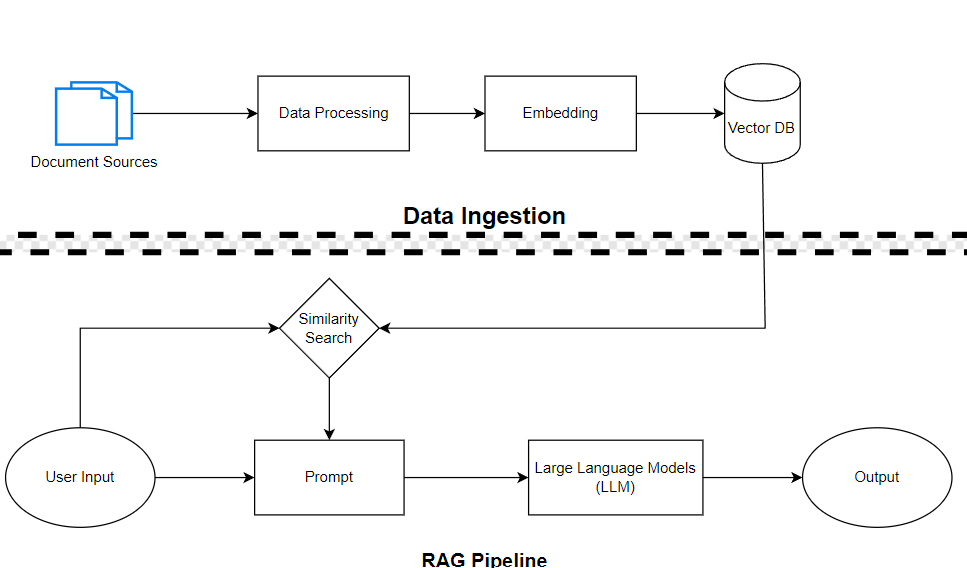
\includegraphics[scale=0.7]{basic_RAG_pipeline.png}
	\end{center}
	\caption{Figure 1: Basic Retrieval-Augmented Generation (RAG) Pipeline (better illustration coming)}
	\label{fig:ascent}
\end{figure}

RAG provides several advantages and solutions to LLMs caveats:
\begin{itemize}
	\item 1. Empowering LLM solutions with real-time data access
	LLMs are typically trained on vast datasets that may quickly become outdated as new information emerges. RAG technology addresses this limitation by allowing LLMs to access and incorporate real-time data into their responses. Through the retrieval component, RAG systems can query up-to-date databases or the internet to find the most current information, ensuring that the generated output reflects the latest developments.
	\item 2. Preserving data privacy
	RAG can retrieve information from a controlled, secure dataset or environment rather than relying on direct access to private data. By designing the retrieval component to operate within privacy-preserving parameters, RAG can ensure that the LLM will not directly access or expose sensitive data.
	\item 3. Mitigating LLM hallucinations
	"Hallucination" in the context of LLMs refers to the generation of plausible but inaccurate or entirely fabricated information. This is a known challenge with LLMs, where the model might confidently produce incorrect data or statements.(cite) RAG helps mitigate this issue by grounding the LLM's responses in retrieved documents that are verified or deemed reliable. By leveraging external sources of information, RAG reduces the model's reliance on potentially flawed internal representations and biases, leading to more accurate outputs.
\end{itemize}

RAG has become very popular since its introduction in Lewis et al. 2020, with its most-known implementation, ChatGPT (powered by GPT-4), creating a sizeable and long-term impact in all industries and academic institutions.
Its versatility in several fields has fueled interest in research and development to develop more RAG implementations. Our package, GRAG (Good RAG), aims to add to the RAG literature.

% ------------------------------------------------------------------------------------------------------------------------
\section{Problem Statement}

While RAG APIs such as OpenAI are very powerful, they usually have usage limits at the free tier, which could be a barrier for extensive commercial use.
Dependence on APIs could limit customization and integration to existing software, which is not ideal for institutions or individuals who have specific needs for their application.
Furthermore, sensitive data being stored on external servers, on top of data usage policy dependent on API providers; raise concerns of data privacy.
GRAG aims to provide a customizable, easy-to-use, end-to-end, open-sourced solution that resolves cost and data privacy issues. The package could be implemented locally, allowing for control over data storage and maximizing personalization.

% ------------------------------------------------------------------------------------------------------------------------

\section{Related Work}


% ------------------------------------------------------------------------------------------------------------------------
\section{Methodology & Features}

\subsection {PDF Parser}
Parsing PDF documents presents a significant challenge due to their complex structure. PDFs often contain unstructured data, which lacks a predefined organization, making accurate recognition and processing arduous. A notable difficulty arises when handling tables, as PDFs do not inherently understand table columns, complicating the task of recognizing table layouts. This complexity is particularly evident in documents like tax forms, which feature intricate nested table structures. Additionally, scanned PDFs require Optical Character Recognition (OCR) tools to convert images back into text, introducing another layer of complexity.

Initially, we tried only using \textit{unstructured.io} and \textit{pdfplumber}, respectively. Neither libraries could consistently parse all PDF files with high accuracy.
The current strategy is to primarily use the \textit{unstructured.io} library for partitioning and parsing.
For documents containing more complex table structures, such as nested tables or tax forms, \textit{pdfplumber} and \textit{pytesseract} are deployed.
The table structures on the documents are detected, then cropped out before the contained text is extracted from the tables.

The results are still inconsistent, however; and more experimentation is needed for a more robust parsing tool for PDFs.

\subsection{Vector Stores}

Vector store or vector database is a type of database that stores data in high-dimensional vectors. This is a crucial component of RAG, storing embeddings for both retrieval and generation processes.
Currently, GRAG supports \textit{Chroma} and \textit{DeepLake}. By default, our embedding model is \textit{instructor-xl}, but any \textit{HuggingFace} embeddings can be used.

\subsection{LLMs}
As explained above, cost and data privacy concerns mean we could not use OpenAI APIs. To run models locally, \textit{llama.cpp} is the best implementation as it uses a low-level language, with extensive backend support, such as CUDA.
Currently, GRAG provides two options to run LLMs locally:

1. Run LLMs using HuggingFace:
This is the easiest way to get started, but does not offer as much flexibility. If using a config file (\textit{config.ini}), simply need to change the \textit{model_name} to the HuggingFace repo id.
If the models are gated, user would need to provide an authentication token.

2. Run LLMs using llama.cpp
\textit{Llama.cpp} offers great flexibility, but its repo is not user-friendly. To streamline the process, we have a script/cookbook for ease of implementation.

GRAG has been tested with Llama2 7b & 13b, Mixtral 8x7b, Gemma 13b, but could support any model from HuggingFace.

\subsection{Multi-vector Retriever}

We built a retriever, which employs a Langchain tool called \textit{multi-vector retriever}.
Instead of representing each document as one vector, one document is represented by multiple vectors, with each vector being a different aspect of the text.
For example, we could split and then embed smaller chunks of a document, which would help embeddings to better carry semantic context.
Our retriever is used to return the most similar chunks from a vectorDB, as well as a linked document or chunk.

\subsection{RAG Features}

\subsubsection{RAG Document Chains}

Document chains are used in Retrieval-Augmented Generation (RAG) to effectively utilize retrieved documents. These chains serve various purposes, including efficient document processing, task decomposition, and improved accuracy.

\textbf{Stuff Chain}

This is the simplest form of document chain. It involves putting all relevant data into the prompt. Given \(n\) documents, it concatenates the documents with a separator, usually \verb|\n\n|.
The advantage of this method is \textit{it only requires one call to the LLM}, and the model has access to all the information at once.
However, one downside is \textit{most LLMs can only handle a certain amount of context}. For large or multiple documents, stuffing may result in a prompt that exceeds the context limit.
Additionally, this method is \textit{only suitable for smaller amounts of data}. When working with larger data, alternative approaches should be used.

\begin{figure}[H]
    \centering
    \includegraphics[width=0.8\textwidth]{path/to/stuff_chain_langchain.jpg}
    \caption{Illustration of Stuff Chain}
    \caption{Illustration of Stuff Chain}
\end{figure}
\href{https://readmedium.com/en/https:/ogre51.medium.com/types-of-chains-in-langchain-823c8878c2e9}{Source}

\textbf{Refine Chain}

The Refine Documents Chain uses an iterative process to generate a response by analyzing each input document and updating its answer accordingly.
It passes all non-document inputs, the current document, and the latest intermediate answer to an LLM chain to obtain a new answer for each document.
This chain is ideal for tasks that involve analyzing more documents than can fit in the model’s context, as it \textit{only passes a single document to the LLM at a time}.
However, this also means it makes significantly more LLM calls than other chains, such as the Stuff Documents Chain. It may \textit{perform poorly for tasks that require cross-referencing between documents} or detailed information from multiple documents.
Pros of this method include \textit{incorporating more relevant context and potentially less data loss} than the MapReduce Documents Chain. However, \textit{it requires many more LLM calls and the calls are not independent}, meaning they cannot be paralleled like the MapReduce Documents Chain.
There may also be dependencies on the order in which the documents are analyzed, thus it might be ideal to provide documents in order of similarity.

\begin{figure}[H]
    \centering
    \includegraphics[width=0.8\textwidth]{refine_chain_langchain.jpg}
    \caption{Illustration of the Refine Chain method.}
\end{figure}
\href{https://readmedium.com/en/https:/ogre51.medium.com/types-of-chains-in-langchain-823c8878c2e9}{Source}

\textbf{Map Reduce Chain}

To process \textit{large amounts of data efficiently}, the MapReduceDocumentsChain method is used.
This involves applying an LLM chain to each document individually (in the Map step), producing a new document. Then, all the new documents are passed to a separate combine documents chain to get a single output (in the Reduce step). If necessary, the mapped documents can be compressed before passing them to the combine documents chain.
This compression step is performed recursively.
This method requires an initial prompt on each chunk of data.
For summarization tasks, this could be a summary of that chunk, while for question-answering tasks, it could be an answer based solely on that chunk. Then, a different prompt is run to combine all the initial outputs.
The pros of this method are that \textit{it can scale to larger documents and handle more documents} than the StuffDocumentsChain. Additionally, \textit{the calls to the LLM on individual documents are independent and can be parallelized}.
The cons are that it \textit{requires many more calls to the LLM} than the StuffDocumentsChain and \textit{loses some information during the final combining call}.

\begin{figure}[H]
    \centering
    \includegraphics[width=0.8\textwidth]{path/to/map_reduce_chain_image.jpg}
    \caption{Illustration of the Map Reduce Chain method.}
\end{figure}
\href{https://readmedium.com/en/https:/ogre51.medium.com/types-of-chains-in-langchain-823c8878c2e9}{Source}

\subsubsection{Prompting}

Each LLM model has their own prompting strategy.

In additional to model-specific prompting, GRAG provides cookbooks to implement custom prompts and few-shot prompts.

\textit{Custom Prompts}: specifically designed inputs that users craft to guide a language model's response in a desired direction. For example, "Could you write a poem in the style of Edgar Allen Poe?"

\textit{Few-Shot Prompts}:

\subsubsection{Other Hyperparameters}
\begin{itemize}
    \item \textbf{Chunk Sizes} --- generally, the smallest chunk size you can get away with.
    \item \textbf{Similarity Score} --- e.g., cosine similarity, a measure used to determine how similar two documents or vectors are.
    \item \textbf{Embedding} --- a representation of text in a high-dimensional vector space, which allows for capturing the semantic meaning of words or phrases.
\end{itemize}

% ------------------------------------------------------------------------------------------------------------------------

\section{Challenges & Future Work}

\subsection{Document Parsing}

While we have made improvements in parsing PDF files, the results are not consistent for different PDF layouts. More experimentation is needed to produce a more robust and accurate result.
We also plan to implement document parsing for other document types, such as .html or .doc.

\subsection{Graph DB implementation}

Traditionally, RAG implementations uses vector databases for its retrieval process. As RAG uses vector embeddings for its processes, vector database is the optimal choice for ease of retrieval and efficiency in similarity search.
However, since RAG simply outputs the closest vector in relation to the query vector, it leaves room for error if the database does not contain relevant information to the input prompt. This makes RAG overly reliant on the quality of the data and the embedding process.
Graph database presents a very promising possibility due to its complex relational network - in theory, this could solve vector DB's limitation.
There is limited existing literature comparing the performance of vector versus graph database in a RAG implementation. This paper aims to experiment with graph database for RAG, and compare its performance to traditional implementation which uses vector databases.

% ------------------------------------------------------------------------------------------------------------------------

\bibliographystyle{IEEEtran}
\bibliography{references}



%------ To create Appendix with additional stuff -------%
%\newpage
%\appendix
%\section{Appendix}
%Put data files, CAD drawings, additional sketches, etc.

\end{document} 